\section{Introduction}
\label{sec:introduction}
%\KZ{This para should talk about why you need slogan in e-commerce. You should
%picture a scenario from user point of view, not from system point of
%view.}
In e-commerce, recommendation systems plays an important role in providing better shopping experience to customers. 
Traditionally, item-based recommendation widely uses user's historical behaviors to recall a small set of most relevant items as candidates, then recommends items with highest weights after scoring with a ranking model. 
A critical limitation of this framework is that it is not driven by user needs in the first place,
which makes it hard for the recommender system to jump out of historical behaviors.
Recently, to further explore user needs and to improve user shopping experience, 
there have been a number of works~\cite{luo2019conceptualize} proposed to build topic-based recommendation.
%by organizing recommended items into topics (or concepts).
A topic is a short, fluent and reasonable phrase implied user interests
that can be directly recommended to users  together with its associated items.
Usually, the topic candidates are built from frequent phrases collected via 
thoroughly analyzing query logs and product titles in order to cover as many user interests as possible.
We then justify the topics based on E-commerce knowledge base
which makes it more reasonable and more convenient to organize items for topics.  
According to typical E-commerce knowledge base,
there are three named entity types:
\emph{Category} (CG), \emph{Property Key} (PK) and \emph{Property Value} (PV).
As shown in \figref{fig:cpv},
``Light fixture" is a Category, 
while ``Material" denotes a Property Key, which is the name of one product property.
``Glass"  and ``Plastic" are concrete property values of ``Material".
We constrain the topic to a phrase which consists of a Category modified by a reasonable Property Value.
Following this constraint, the topic can be associated with 
a set of items belong to the Category with the corresponding Property Value.
For example, ``glass light fixture" is a satisfied topic,
which the Category ``light fixture" is modified
by the concrete Property Value ``glass" of its 
corresponding product property ``Material".
Note that, ``Tools for baking" in \figref{fig:cpv}
also represents a topic which can be seen a Category modified by an empty Property Value.  
\begin{figure}[th!]
	\centering
	\includegraphics[width=0.95\columnwidth]{figures/cpv2}
	\caption{The structure of E-commerce knowledge-base.}
	\label{fig:cpv}
\end{figure}

The topic-based recommendation organizes items as topics implied user interests 
which provides superior shopping experience to users as well as recommends in a more efficient way.
Taobao App incorporates the topic-based recommendation 
into recommendation system to satisfy the scenario of coarse-grained recommendation.
%As shown in \figref{fig:topic} \textbf{PLACEHOLDER},
%the topic ``glass light fixture" is displayed to users as a card with
%its textual description and the picture of a representative item (left).
%Once a user clicks on it, he will enter into another page (right) where
%different items satisfied the needs of ``glass light fixture" are displayed.
As we can see that textual descriptions are like salespeople,
that is critical to demonstrate the recommended topics to customers.
Quality textual descriptions attract users' attention, promote users' interests and eventually convince users to buy the recommended products.
However, until now, most of the textual descriptions for topics in the online shopping platforms,
namely \emph{slogan},
are still created manually, 
which is tedious, time-consuming, and less effective.
On the other hand, such slogans should be personalized based on the item preferences
which highlights the selling points to users
and promotes their interests accordingly.
In this paper, we focus on automating the slogan generation
for online shopping in E-commerce.
%We formulate it as a text-to-text generation problem.
Specially, the system can intelligently generate an accurate and
attractive slogan for a specific topic based on the given topic information and item preferences.

\begin{figure*}[th!]
	%	\small
	\centering
	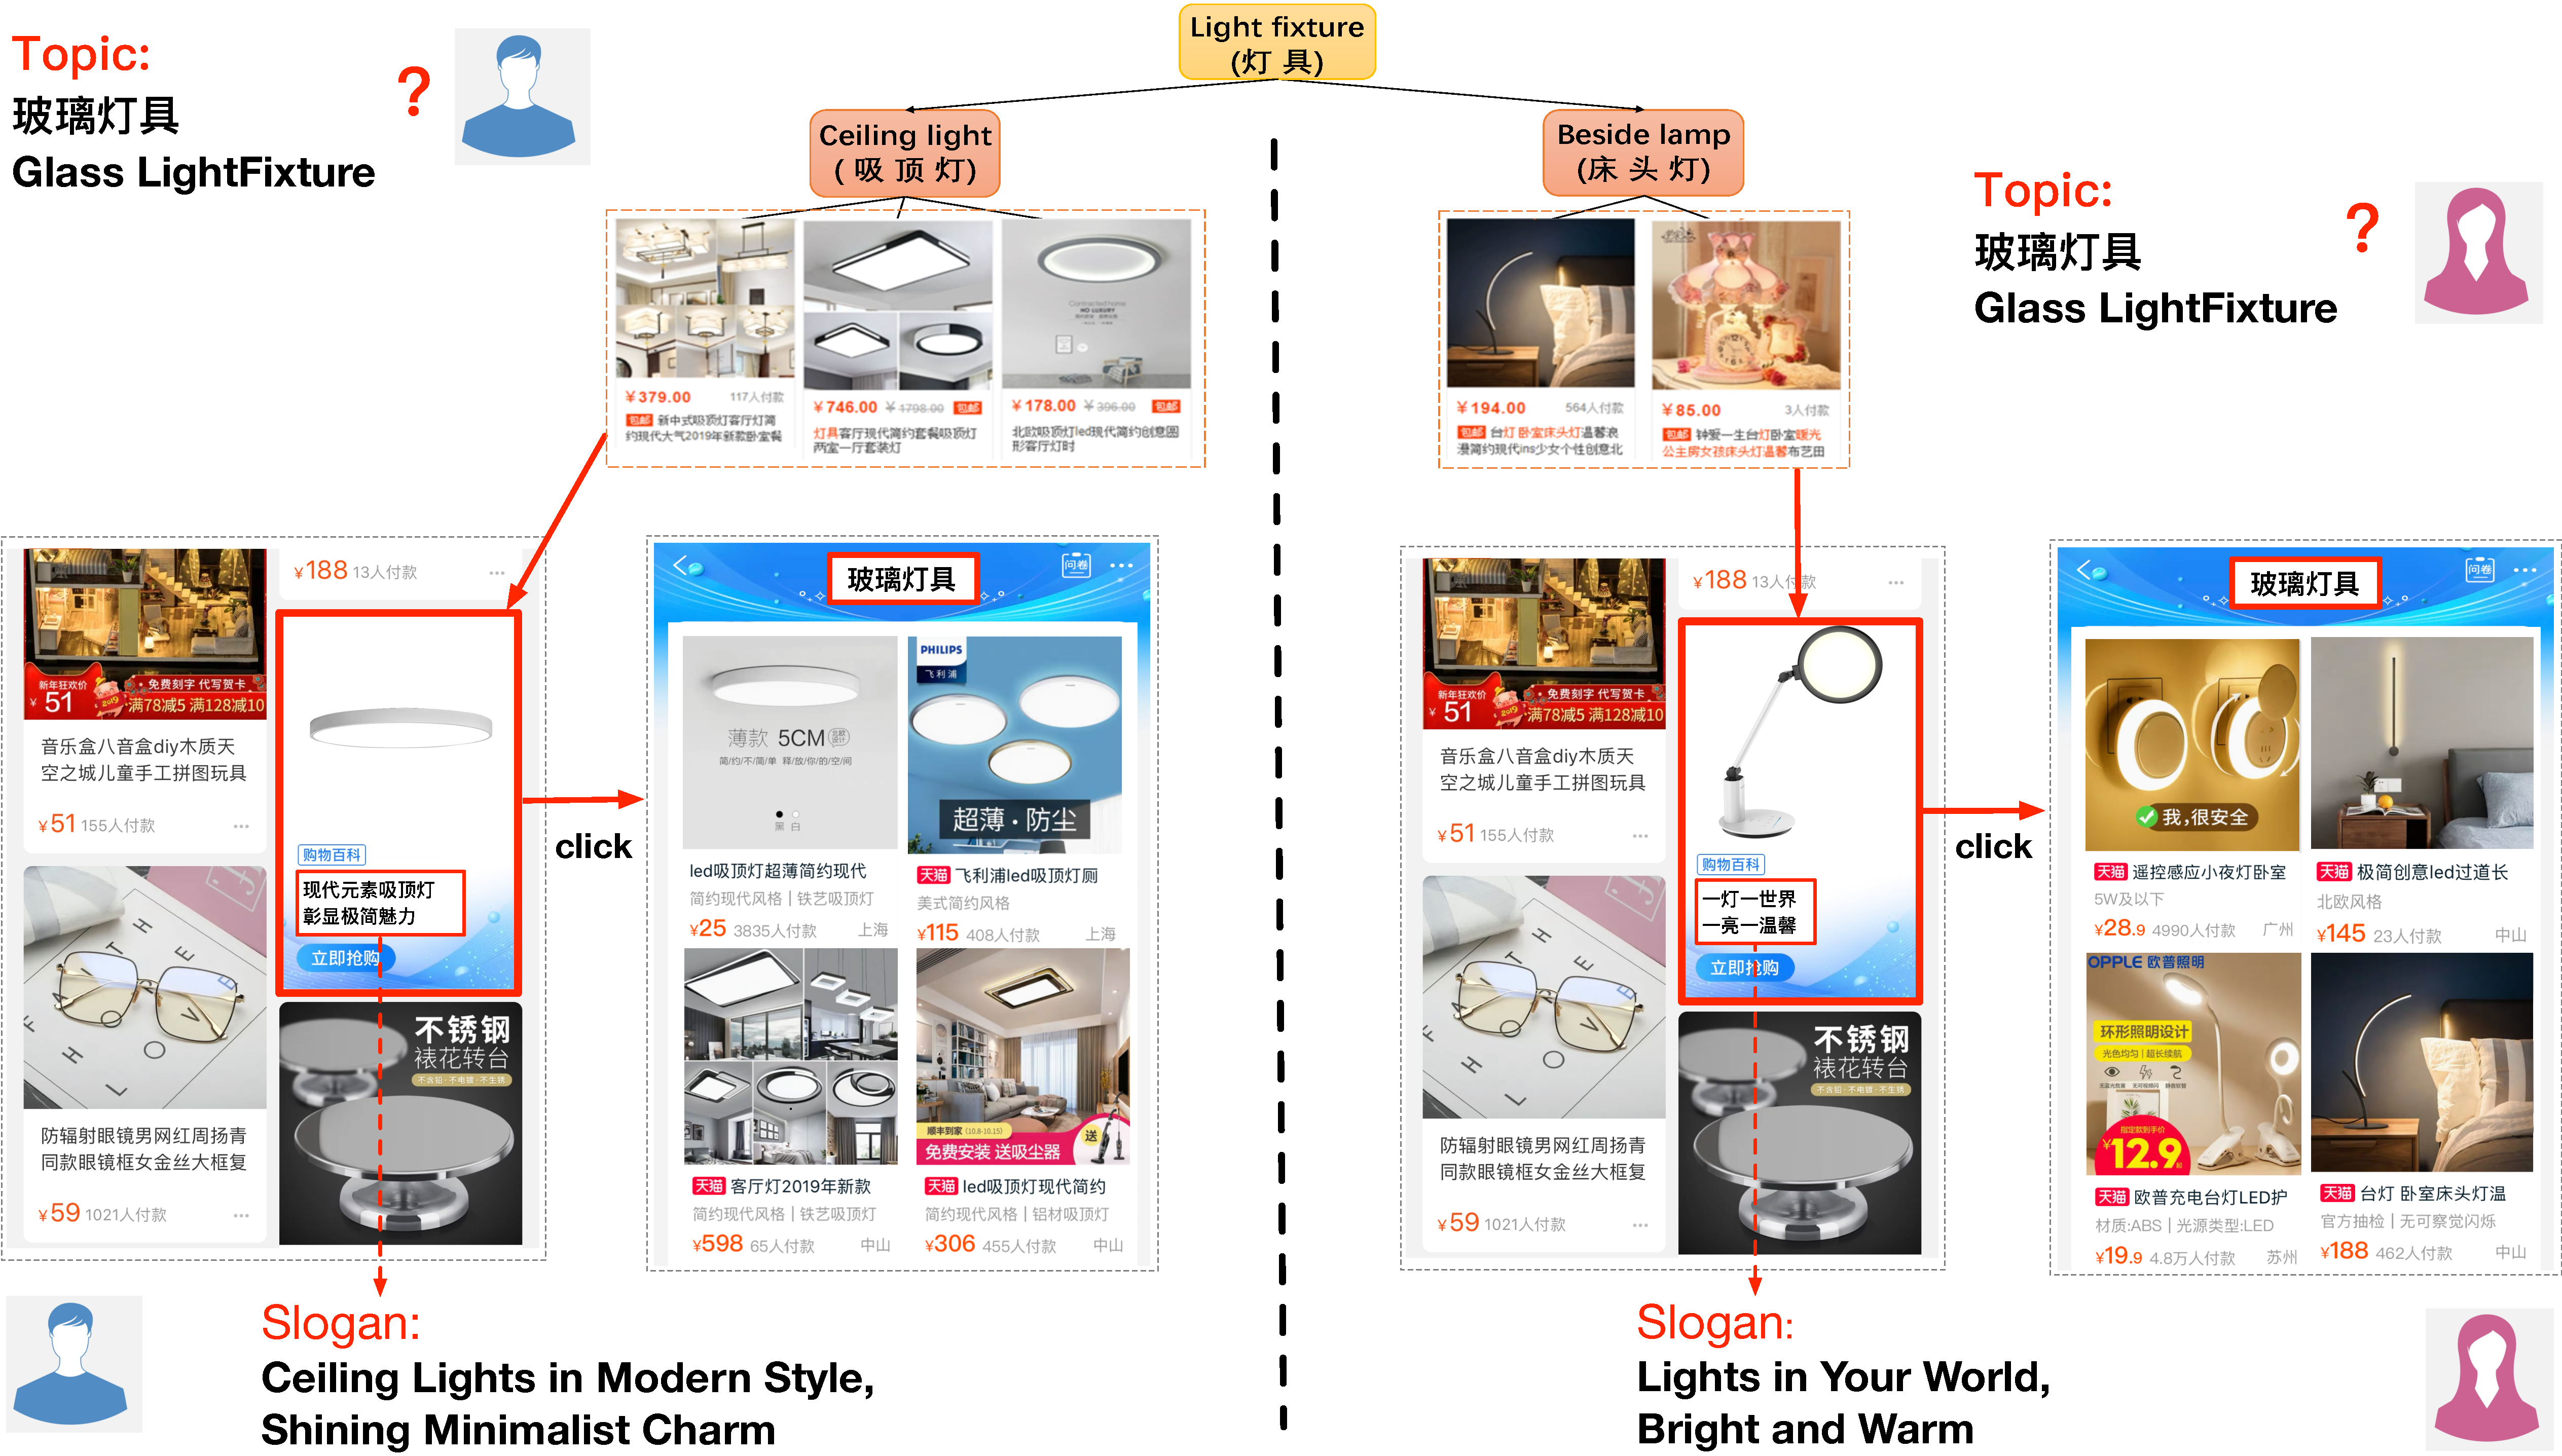
\includegraphics[width=1.9\columnwidth]{figures/cloud}
	\caption{An motivating example of slogan generation in e-commerce.
		Two item preferences are introduced for a specific topic ``glass light fixture" using category ontology (top). The topic associated with a preference is displayed to users as a card with its textual description and the picture of a representative item. Once a user clicks on it, he will enter into another page where different items satisfied the preference are displayed. }
	\label{fig:cloud}
\end{figure*}


Slogan generation in E-commerce is a relative new problem.
The most related work is E-commerce product title generation
which aims to present products using titles to summarize product information.
Existing works on title generation are mostly 
selection-based and statistical-based.
In the case of selection-based approaches, 
Cillick~\cite{gillick2011elements} adapts the diversity-based ranking techniques in extractive summarization to title generation, pruning and selecting the title from a set of title candidates.
Moreover, the systems~\cite{rosti2007improved,barrault2010many,mathur2017generating,suzuki2011automatic} can also learn how to pick the candidate title which is closest to the reference title.
Souza et al.~\cite{de2018generating} statistics about the item titles and
recombine frequent n-grams as generated titles using a stack-based search algorithm. 
Another relevant work is the product description generation task in E-commerce.
Most prior works are based on templates and traditional statistical frameworks
~\cite{langkilde1998generation,wang2017statistical} which are insufficient to generate personalized and informative descriptions.
%Product descriptions usually are longer than slogans, thus rely on 
Recently, Chen et al.~\cite{ChenLZYZ019} extend the encoder-decoder framework
to product description generation and achieve better performance. 

%We formulate personalized slogan generation as a text-to-text generation task.
%Owing to the tremendous success of
Crafting a successful slogan for specific topic is tedious and highly time-consuming.
Besides, previous related works are mainly use templates or statistical methods
which are insufficient to achieve satisfying performance.
On the other hand, convolutional sequence-to-sequence (Seq2Seq) learning has been achieved tremendous success in many text generation applications,
such as machine translation~\cite{wang2017statistical,chen2018stable,song2018double,wu2019pay},
abstractive document summarization~\cite{fan2017controllable,liu2018controlling,narayan2018don},
language modeling~\cite{baevski2018adaptive},
story generation~\cite{fan2018hierarchical,fan2019strategies}
and dialogue~\cite{miller2017parlai,dinan2018wizard}.
Owing to this success, we propose a \textbf{S}emantics-enh\textbf{A}nced
s\textbf{L}ogan gen\textbf{E}ration (or SALE) model for online topic-based recommendation.
We extend the effective convolutional Seq2Seq framework~\cite{ott2019fairseq}
to slogan generation.
SALE introduces the item preferences for topics using category ontology
in order to generate more attractive slogans which highlight diverse focuses or selling-points.
Moreover, SALE incorporates \emph{is-a} knowledge
from an external knowledge base and
also integrates potential commonsense knowledge from pre-trained language model for robustness at inference.
%\figref{fig:cloud} shows an example of semantics-enhanced
%slogan generation in E-commerce.
%[用一个大图替换掉 \figref{fig:cate}]
 
% A product title is the realization of this information in a human-readable way so that users can understand the main features of the product.

To provide a dataset for the automatic slogan generation,
we construct and make publicly available a new dataset from Taobao.
We collect 857 topics and in total 3,555 pairs of topic provided with a item preference
and manually created slogan accordingly.
An item preference is represented as a set of items sampled from secondary categories 
associating to a specific topic.
We further illustrate this in details in \secref{sec:preference}.
We also retrieve the \emph{is-a} knowledge
from a external knowledge base in Chinese.
The involved \emph{is-a} knowledge will be released together with previous created dataset.
Models trained on the dataset are able to learn how to generate slogans based on topics,
item preferences and relevant knowledge.

The contributions of this paper are summarized below:
\begin{itemize}
	\item We define a new problem personalized slogan generation, 
	generating accurate and attractive slogans,which benefits existing
	recommendation systems in E-commerce.
	\item We propose a novel model SALE based-on sequence-to-sequence learning, 
	which utilizes item preferences for personalization and further incorporates the hypernym-hyponym semantic knowledge as well as potential commonsense knowledge to improve the quality of generation. Extensive experiments show that our approach outperforms several baselines by a substantial margin.
	\item We create a new dataset for automatic slogan generation (\secref{sec:eval_dataset}).
	We intend to release this dataset as well as the implementation of the proposed method for future work in this research area. 
\end{itemize}


%we build various preferred item sets for topics to represent users' preferences accordingly
%by introducing category ontology in E-commerce.
%Such item sets reflect different focuses and potential interests of users.

%讲一下personalize
%users needs - topic - items
%user preferences - secondary category - items


%The most related work are about product description generation and 
%title generation for browse pages.
%
%We introduce the category ontology 
%In topic-based recommendation, a topic bridges user needs and its associated items.
%Similarly, user preferences to a specific topic can be expressed by  
%Similarly, category ontology is introduced as potential focuses
%connecting user preference and items.





%It is necessary to make the slogan focuses adapted to 
%the selling points conducting by users' preferences of items.
%
%A set of associated items represents the users' needs
%by summarizing and con
%A set of preferred items which relevant to a specific topic
%can represent the users' preferences 
%It is reasonable to represent the users' preferences
%of a specific topic as a set of preferred items
%which are relevant to the topic. 
%Besides, such item preferences 
%Different from exploring users' preference from private information,
%we represent the preferences as a set of preferred items relevant to
%a specific topic.
%The system is expzected to explore selling points from 
%the topic and the provided preferred items,

%\begin{figure}[th!]
%	\centering
%	\includegraphics[width=0.95\columnwidth]{figures/cate8}
%	\caption{An example of category structure in E-commerce.}
%	\label{fig:cate}
%\end{figure}




%One of the biggest challenges of recommendation in E-commerce is to 
%efficiently  in an accurate and attractive way.


%说为topic生成标题的重要性

%item-specific details
%attract customer's attention and transfer it to purchase
%别人是怎么做的 局限性在哪


%In this paper, 
%我们要做的是啥
%说明下我们的topic是啥
%我们准备怎么做

%最后总结一下我们的贡献是啥

%related work
%item-based recommendation 展示: product description generation
%topic-based recommendation 展示: slogan generation

%E-commerce platforms traditionally present and recommend items to users using titles and demo pictures from on-line merchants that describe items information.  
% limitations

%To resolve these limitations, instead of \emph{item-based} presentation and recommendation, recent works focus on exploring user needs and propose \emph{topic-based} presentation and recommendation~\cite{}.



%[ebay emnlp 2018] Generating E-Commerce Product Titles and Predicting their Quality
%[kdd 2019] Towards Knowledge-Based Personalized Product Description Generation in E-commerce
%[ICML 2019] Generative Adversarial User Model for Reinforcement Learning Based Recommendation System
